\documentclass[tikz,border=6pt]{standalone}
\usepackage{pgfplots}
\pgfplotsset{compat=1.18}
\usepgfplotslibrary{colormaps}
\usetikzlibrary{arrows, arrows.meta, calc}
\usetikzlibrary{decorations.markings}


\usepackage{amssymb,amsmath,mathtools}

\usepackage[T1]{fontenc}
\usepackage[utf8]{inputenc}
\usepackage{newpxtext,newpxmath}
\usepackage{sectsty}

\renewcommand{\Re}{\operatorname{\mathrm{Re}}}
\renewcommand{\Im}{\operatorname{\mathrm{Im}}}

\begin{document}
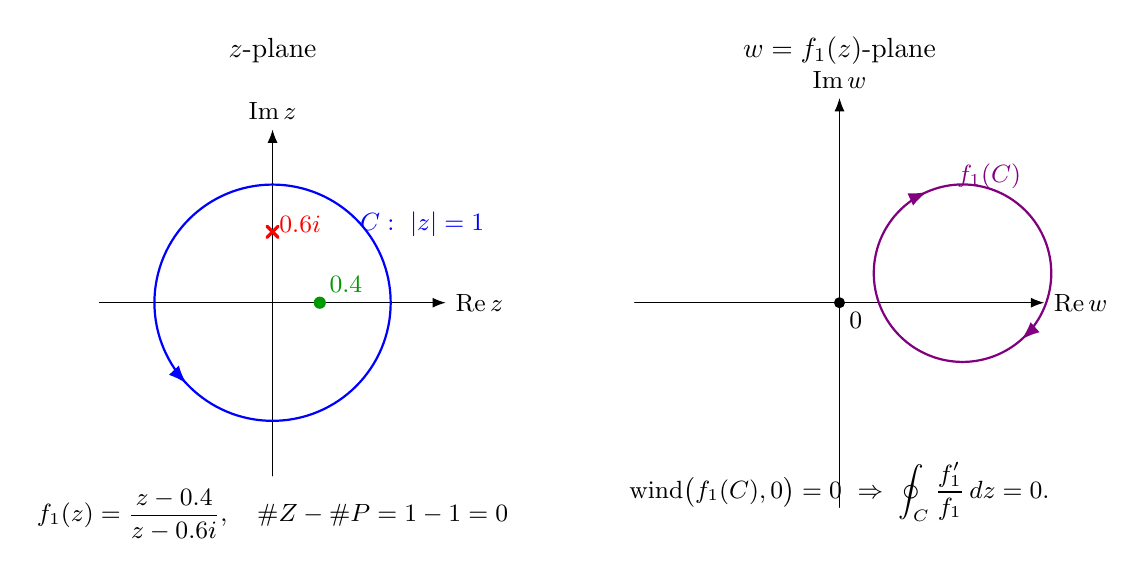
\begin{tikzpicture}[>=Latex, line cap=round, line join=round, font=\small]

% ==== Left: z-plane ====
\begin{scope}
	\node[font=\normalsize] at (0,3.2) {$z$-plane};
	\draw[->] (-2.2,0)--(2.2,0) node[right] {$\Re z$};
	\draw[->] (0,-2.2)--(0,2.2) node[above] {$\Im z$};
	
	% unit circle C
	\draw[blue,thick,postaction={decorate},
	decoration={markings, mark=at position 0.62 with {\arrow{>}}}]
	(0,0) circle (1.5);
	\node[blue] at (1.9,1.0) {$C:\ |z|=1$};
	
	% zero inside
	\fill[green!60!black] (0.6,0) circle(2.2pt) node[above right] {$0.4$};
	% pole inside
	\draw[red,very thick] (0,0.9) ++(-0.07,-0.07) -- ++(0.14,0.14);
	\draw[red,very thick] (0,0.9) ++(-0.07,0.07) -- ++(0.14,-0.14);
	\node[red] at (0.35,1.0) {$0.6i$};
	
	\node[align=left] at (0,-2.7) {$\displaystyle
		f_1(z)=\frac{z-0.4}{z-0.6i},\quad \#Z-\#P=1-1=0$};
\end{scope}

% ==== Right: w-plane ====
\begin{scope}[shift={(7.2,0)}]
	\node[font=\normalsize] at (0,3.2) {$w=f_1(z)$-plane};
	\draw[->] (-2.6,0)--(2.6,0) node[right] {$\Re w$};
	\draw[->] (0,-2.6)--(0,2.6) node[above] {$\Im w$};
	\fill (0,0) circle(2pt) node[below right] {$0$};
	
	% f(e^{it}) with x=cos t, y=sin t
	\draw[violet,thick,
	postaction={decorate},
	decoration={markings, mark=at position 0.20 with {\arrow{>}},
		mark=at position 0.65 with {\arrow{>}}}]
	plot[domain=0:6.283, samples=500] 
	({
		% Re f = (N_re*D_re + N_im*D_im)/|D|^2
		% N = (x-0.4) + i y
		% D = x + i(y-0.6)
		((cos(\x r)-0.4)*cos(\x r) + (sin(\x r))*(sin(\x r)-0.6)) /
		(cos(\x r)*cos(\x r) + (sin(\x r)-0.6)*(sin(\x r)-0.6))
	},
	{
		% Im f = (N_im*D_re - N_re*D_im)/|D|^2
		( (sin(\x r))*cos(\x r) - (cos(\x r)-0.4)*(sin(\x r)-0.6) ) /
		(cos(\x r)*cos(\x r) + (sin(\x r)-0.6)*(sin(\x r)-0.6))
	});
	\node[violet] at (1.9,1.6) {$f_1(C)$};
	
	\node[align=center] at (0,-2.4)
	{$\mathrm{wind}\big(f_1(C),0\big)=0
		\ \Rightarrow\ 
		\displaystyle \oint_C \frac{f_1'}{f_1}\,dz=0.$};
\end{scope}

\end{tikzpicture}
\end{document}
